\subsection{Dasbor Pengawasan}

Terdapat berbagai dasbor Grafana yang disiapkan untuk memudahkan proses pengawasan pada kluster tiket dan kluster penguji. Sebagian besar dasbor ini merupakan dasbor bawaan dan buatan komunitas yang diambil dari galeri dasbor Grafana atau kakas yang berkaitan. Sebagai contoh, Gambar \ref{fig:ticket-dashboard-example} menunjukkan tampilan salah satu dasbor pengawasan yang digunakan selama pengujian.

\begin{figure}[H]
    \centering
    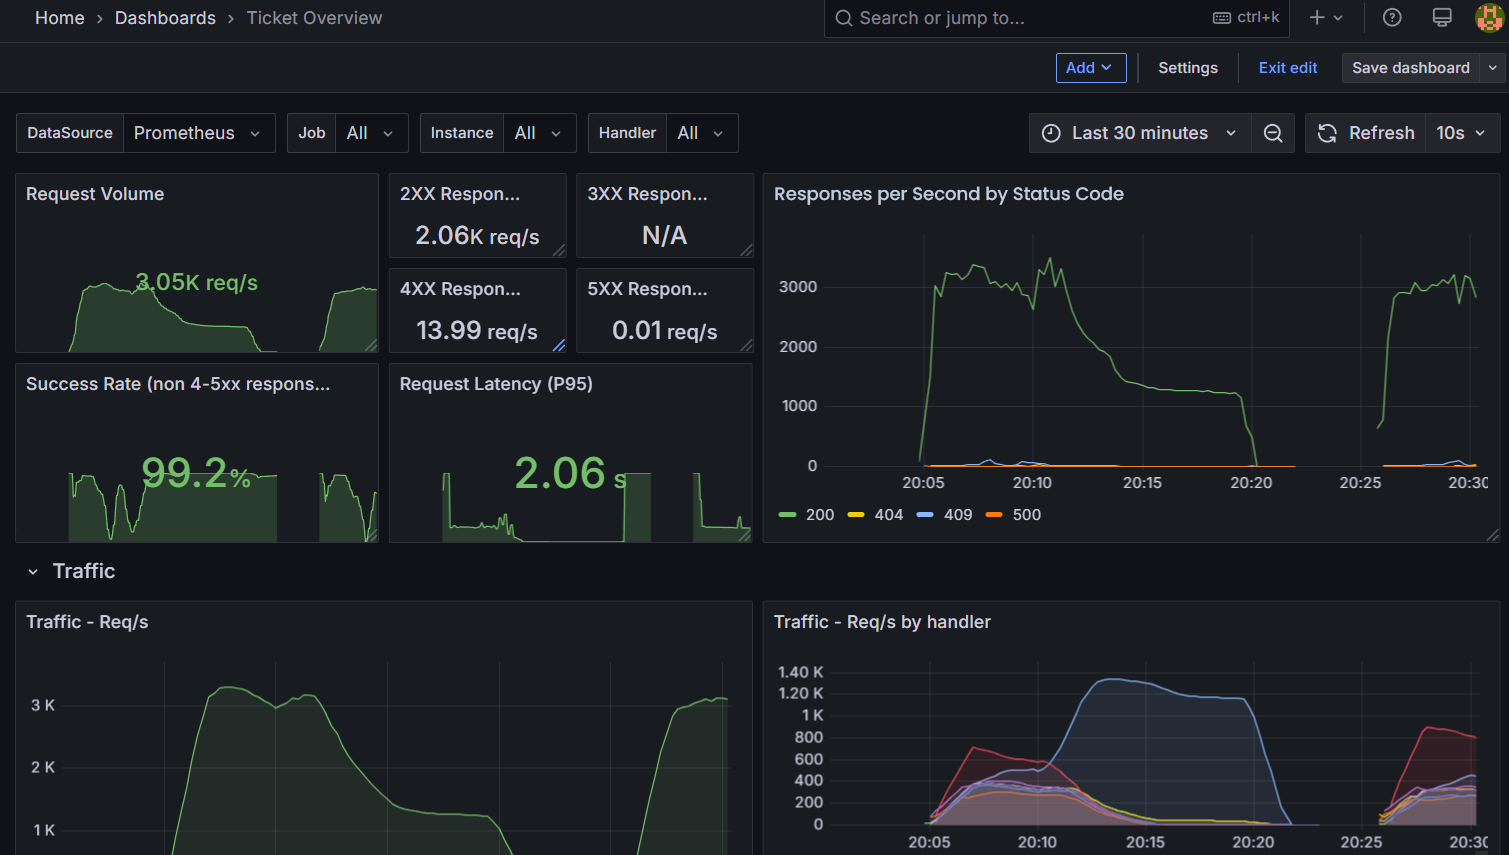
\includegraphics[width=1\textwidth]{resources/chapter-4/ticket-dashboard.png}
    \caption{Contoh Dasbor Layanan Tiket}
    \label{fig:ticket-dashboard-example}
\end{figure}

Selain itu, terdapat dasbor yang menampilkan \textit{log} aplikasi sebagaimana ditunjukkan pada Gambar \ref{fig:log-example}. Dasbor ini digunakan juga untuk mengawasi keberjalanan pengujian dan menentukan apakah terjadi kegagalan yang tidak diduga selama pengujian. Rincian lengkap dasbor pengawasan disertakan pada Lampiran \ref{apx:monitoring-dashboard}.

\begin{figure}[H]
    \centering
    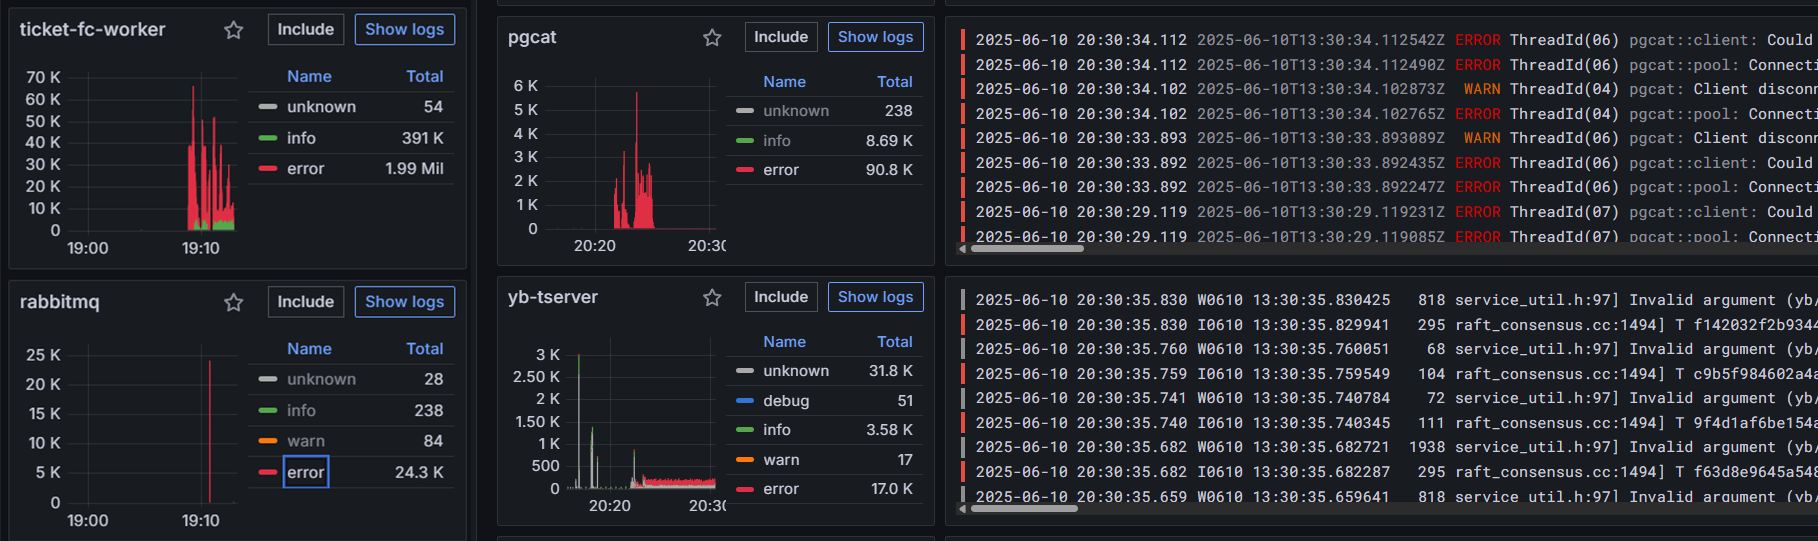
\includegraphics[width=1\textwidth]{resources/chapter-4/log.png}
    \caption{Contoh \textit{Log} Sistem Tiket}
    \label{fig:log-example}
\end{figure}
